\section{Empirical phase-continuation tensor}
\label{sec:empirical-tensor}

The controlled domain studies establish that continuation can distinguish smooth
crossovers from finite-size sharpening, but they do not by themselves identify
which choices in a modern Transformer move a boundary.  We therefore factor the
Transformer study into a phase-continuation tensor
\begin{equation}
  \mathcal{T}=
  \mathcal{D}\times\mathcal{A}\times\mathcal{F}\times\mathcal{R}
  \times\mathcal{O}\times\mathcal{U}\times\mathcal{S}
  \times\mathcal{C}\times\mathcal{P},
\end{equation}
whose coordinates are data, attention, MLP, residual parameterization,
learning objective, optimizer, scaling path, lifecycle, and population.  This
factorization changes the empirical question from ``does a Transformer have a
phase transition?'' to the falsifiable question ``which boundary, measured by
which intensive observable, is transported when one coordinate is continued
while the others are held fixed?''  The distinction is important because width,
depth, context, and data are inequivalent scaling paths, and optimizer rankings
can reverse under normalization or learning-rate changes.

\subsection{Coverage is a result, not a footnote}

The tensor is a taxonomy rather than an assertion that every Cartesian-product
cell has been run. Figure~\ref{fig:tensor-coverage} records the evidence tier
of each coordinate and leaves untested cells visibly marked as N0. The present
trainable program covers the MLP, residual/normalization, objective, optimizer,
and scaling edges on controlled synthetic data; the data edge additionally has
semi-natural and bounded natural-corpus endpoints. Attention is represented by
the solvable and reduced numerical anchors developed in the preceding sections,
whereas lifecycle and population continuations remain protocols rather than
empirical claims in this Transformer bridge.

\begin{table}[t]
\centering\small\setlength{\tabcolsep}{4pt}
\begin{tabular}{lll}
\toprule
Coordinate & Registered primary observable & Current evidence tier \\
\midrule
Data $\mathcal D$ & $s(\mathcal D),R_{\rm test},e_{\rm OOD}$ & N2, R1, R2 \\
Attention $\mathcal A$ & $m_{\rm att}$, head response & T0, T1, N1 \\
MLP $\mathcal F$ & $\Delta_{\rm MLP}$, $\mathrm{PR}_{\rm MLP}$ & N2 \\
Residual $\mathcal R$ & stream RMS, depth correlation & N2 \\
Objective $\mathcal O$ & $\tilde\ell$, Brier, alignment & N2 \\
Optimizer $\mathcal U$ & $G_{\rm block}$, noise scale & N2 \\
Scaling $\mathcal S$ & $R_{\rm test}(N_{\rm path})$ & T1, N2 \\
Lifecycle $\mathcal C$ & drift and transfer response & N0 \\
Population $\mathcal P$ & effective multiplicity & N0 \\
\bottomrule
\end{tabular}
\caption{Nine-axis coverage matrix. T0/T1 are exact/asymptotic theory,
N1/N2 reduced/trainable synthetic numerics, R1/R2 semi-natural/natural data,
and N0 explicitly denotes an untested cell.}
\end{table}

\subsection{Trainable bridge and dimensionless observables}

The bridge model is a causal byte-level decoder with tied embeddings, explicit
multi-head causal attention, configurable pre/post LayerNorm or RMSNorm, and an
MLP selected from no MLP, linear, ReLU, GELU, GEGLU, and SwiGLU.  The fixed
258-symbol vocabulary makes natural-corpus risks comparable in bits per byte,
without a tokenizer-dependent denominator.  Synthetic retrieval, counting, and
hidden-state sources provide known interventions; bounded TinyStories,
SimpleStories, FineWeb-Edu, and Dolma samples test boundary transport to natural
data.  Natural-corpus comparisons are distributional stress tests rather than
claims about frontier-scale language modelling.

All reported performance observables are $O(1)$ under the intended continuation.
For a vocabulary of size $V$, we separately report
\begin{equation}
R_{\rm train}=\ell_{\rm train}/\log V,\qquad
R_{\rm test}=\ell_{\rm test}/\log V,\qquad
R_{\rm OOD}=\ell_{\rm OOD}/\log V,\qquad
e_{\rm gen}=R_{\rm test}-R_{\rm train}.
\end{equation}
Thus a held-out risk is never called a generalization gap. Brier risk is divided
by its vocabulary-scale reference. Attention entropy is divided by $\log L$,
MLP participation ratio and local Jacobian participation ratio by MLP width, and
activation entropy by the logarithm of that width. Activation sparsity, gated-unit
saturation, residual-stream RMS, token-mean drift, nearest-layer correlation,
two-minibatch gradient-noise scale, and corpus summary statistics are reported as
mechanism diagnostics; they do not substitute for a risk metric. The sample path is
\begin{equation}
  N_{\rm train}=\min\{N_{\rm cap},\lceil\alpha d^{\gamma}\rceil\},
\end{equation}
so $\alpha$ is a dimensionless control while $\gamma$ distinguishes data-scaling
paths.  Compute, parameter count, tokens, and wall time are retained as
extensive audit coordinates, never substituted for an intensive order
parameter.  This follows the separation between model scaling and data scaling
in compute-optimal training and the need for parameterization-aware transfer
across widths~\cite{tensor_chinchilla_hoffmann2022,tensor_mup_yang2022}.

\subsection{Optimizer geometry, causal decomposition, and statistics}

We compare SGD with momentum, AdamW, Muon, SOAP, Lion, and GaLore.  Learning rate
is itself swept for the primary SGD--AdamW--Muon--SOAP comparison and crossed
with pre-RMSNorm, pre-LayerNorm, and post-LayerNorm; conclusions are therefore
based on response surfaces rather than vendor defaults.  Muon acts only on
internal two-dimensional weight matrices, while embeddings, readout weights,
biases, and scale parameters use AdamW.  This respects the optimizer's matrix
geometry rather than silently applying it to semantically different parameter
blocks~\cite{tensor_muon_jordan2025,tensor_soap_vyas2024,tensor_galore_zhao2024}.

Attention and MLP contributions are measured by paired inference-time
interventions on the same trained checkpoint.  If $R$, $R_{-A}$, $R_{-M}$, and
$R_{-AM}$ denote intensive risks for the full, attention-ablated, MLP-ablated,
and doubly ablated networks, respectively, we report
\begin{align}
  \Delta_A &= R_{-A}-R, &
  \Delta_M &= R_{-M}-R, &
  \Delta_{AM} &= R_{-AM}-R_{-A}-R_{-M}+R.
\end{align}
These interventions separate functional dependence from attention-map
appearance. Gradient-block Gini coefficient, log-scale coefficient of variation,
two-minibatch gradient-noise scale, update-to-weight RMS, normalized participation
ratios, and time to cross the task-order threshold provide mechanism-resolving
diagnostics. At every registered checkpoint, five-seed train/test trajectories are
aggregated before plotting; a final-score improvement that does not persist in
$e_{\rm gen}$ is therefore not interpreted as improved generalization.

Every confirmatory condition uses exactly the same five distinct seeds.  A seed
controls data generation or corpus windows, initialization, minibatch order,
dropout, and evaluation through stable nested hashes.  Error bars are two-sided
95\% Student-$t$ intervals over the five full pipelines ($t_{4,0.975}=2.776$).
For each seed, a boundary is linearly interpolated at semantic order $m=1/2$;
the five boundary estimates, rather than pooled checkpoints, are then averaged.
Aggregation fails if even one seed is absent or non-finite.  This avoids both
pseudoreplication and understated uncertainty near a steep crossover.

\subsection{Orthogonal continuation results}

Figures~\ref{fig:tensor-mlp-phase}--\ref{fig:tensor-mlp-mechanism} are generated only
from the immutable five-seed aggregate.  Their roles are deliberately
non-redundant: MLP family and causal division of labour, optimizer geometry and
gradient heterogeneity, objective homotopy, inequivalent scaling paths,
synthetic-to-natural transport, and the compute--error envelope.  Together with
the diffusion, reinforcement-learning, and multi-agent anchors above, they form
one taxonomy: the Transformer is the mechanism-rich flagship, while the other
domains test whether the same continuation protocol survives a change of
microscopic semantics.

\IfFileExists{generated/phase_tensor_results.tex}{
% Generated from the strict manifest-seed aggregate; do not edit by hand.
\providecommand{\AdamWError}{$0.541\pm 0.010$}
\providecommand{\AdamWGini}{$0.521\pm 0.030$}
\providecommand{\AdamWLearningRate}{0.0003}
\providecommand{\AdamWLearningRateCalibrationAlpha}{0.5}
\providecommand{\AdamWLearningRateCalibrationSize}{64}
\providecommand{\AdamWLearningRateSelectionStatus}{calibrated (d=64, alpha=0.5)}
\providecommand{\DolmaBitsPerByte}{$3.257\pm 0.057$}
\providecommand{\DolmaSemanticOrder}{$0.593\pm 0.007$}
\providecommand{\FineWebEduBitsPerByte}{$3.427\pm 0.044$}
\providecommand{\FineWebEduSemanticOrder}{$0.572\pm 0.005$}
\providecommand{\LinearDataScalingError}{$0.812\pm 0.031$}
\providecommand{\MLPGEGLUOrder}{$0.433\pm 0.037$}
\providecommand{\MLPGELUOrder}{$0.515\pm 0.017$}
\providecommand{\MLPNoneOrder}{$0.548\pm 0.011$}
\providecommand{\MLPSwiGLUOrder}{$0.435\pm 0.047$}
\providecommand{\MuonError}{$0.537\pm 0.005$}
\providecommand{\MuonGini}{$0.540\pm 0.014$}
\providecommand{\MuonLearningRate}{0.0003}
\providecommand{\MuonLearningRateCalibrationAlpha}{0.5}
\providecommand{\MuonLearningRateCalibrationSize}{64}
\providecommand{\MuonLearningRateSelectionStatus}{calibrated (d=64, alpha=0.5)}
\providecommand{\PhaseTensorBoundaries}{386}
\providecommand{\PhaseTensorConditions}{1,740}
\providecommand{\PhaseTensorRuns}{8,700}
\providecommand{\QuadraticDataScalingError}{$0.394\pm 0.010$}
\providecommand{\SGDMError}{$0.622\pm 0.002$}
\providecommand{\SGDMGini}{$0.629\pm 0.025$}
\providecommand{\SGDMLearningRate}{0.003}
\providecommand{\SGDMLearningRateCalibrationAlpha}{0.5}
\providecommand{\SGDMLearningRateCalibrationSize}{64}
\providecommand{\SGDMLearningRateSelectionStatus}{calibrated (d=64, alpha=0.5)}
\providecommand{\SOAPError}{$0.821\pm 0.009$}
\providecommand{\SOAPGini}{$0.569\pm 0.013$}
\providecommand{\SOAPLearningRate}{0.0003}
\providecommand{\SOAPLearningRateCalibrationAlpha}{0.5}
\providecommand{\SOAPLearningRateCalibrationSize}{64}
\providecommand{\SOAPLearningRateSelectionStatus}{calibrated (d=64, alpha=0.5)}
\providecommand{\SimpleStoriesBitsPerByte}{$2.774\pm 0.063$}
\providecommand{\SimpleStoriesSemanticOrder}{$0.654\pm 0.008$}
\providecommand{\ThreeHalfDataScalingError}{$0.404\pm 0.008$}
\providecommand{\TinyStoriesBitsPerByte}{$2.642\pm 0.089$}
\providecommand{\TinyStoriesSemanticOrder}{$0.670\pm 0.011$}

\paragraph{Observed boundary transport.}
The strict aggregate contains \PhaseTensorRuns{} independently trained runs,
\PhaseTensorConditions{} five-seed conditions, and \PhaseTensorBoundaries{}
per-seed interpolated boundary estimates.  At $d=192$ and $\alpha=8$ on
retrieval, removing the MLP gives semantic order \MLPNoneOrder, compared with
\MLPGELUOrder{} for GELU, \MLPGEGLUOrder{} for GEGLU, and
\MLPSwiGLUOrder{} for SwiGLU.  Thus this task is attention-dominant at the
measured endpoint: adding a gated MLP does not monotonically improve order, and
the MLP family genuinely splits the continuation rather than acting as a proxy
for parameter count.

Under pre-RMSNorm and the learning-rate selection rule defined above, the
intensive errors are \MuonError{} for Muon and \AdamWError{} for AdamW; their
intervals overlap.  By contrast, SGD-M gives \SGDMError{} and SOAP gives
\SOAPError{}.  The corresponding gradient-block Gini coefficients are
\MuonGini, \AdamWGini, \SGDMGini, and \SOAPGini, respectively.  The result is
not a universal optimizer ranking: it is evidence that update geometry and
gradient heterogeneity move together on this controlled bridge, while the
Muon--AdamW endpoint difference is unresolved at five seeds.

The scaling continuation gives the clearest qualitative split.  At $d=192$
and $\alpha=4$, $N\propto d$ yields error \LinearDataScalingError, whereas
$N\propto d^{3/2}$ and $N\propto d^2$ yield
\ThreeHalfDataScalingError{} and \QuadraticDataScalingError.  Width growth at
fixed optimization budget is therefore not interchangeable with data growth.
On natural text with SwiGLU, the same byte-level protocol gives
\TinyStoriesBitsPerByte{} bits/byte on TinyStories,
\SimpleStoriesBitsPerByte{} on SimpleStories, \DolmaBitsPerByte{} on Dolma,
and \FineWebEduBitsPerByte{} on FineWeb-Edu.  These values establish transport
of the measurement protocol, not universality of the numerical boundary.
}{}

\IfFileExists{figures/figure09_mlp_phase_splitting.pdf}{
\begin{figure}[t]
  \centering
  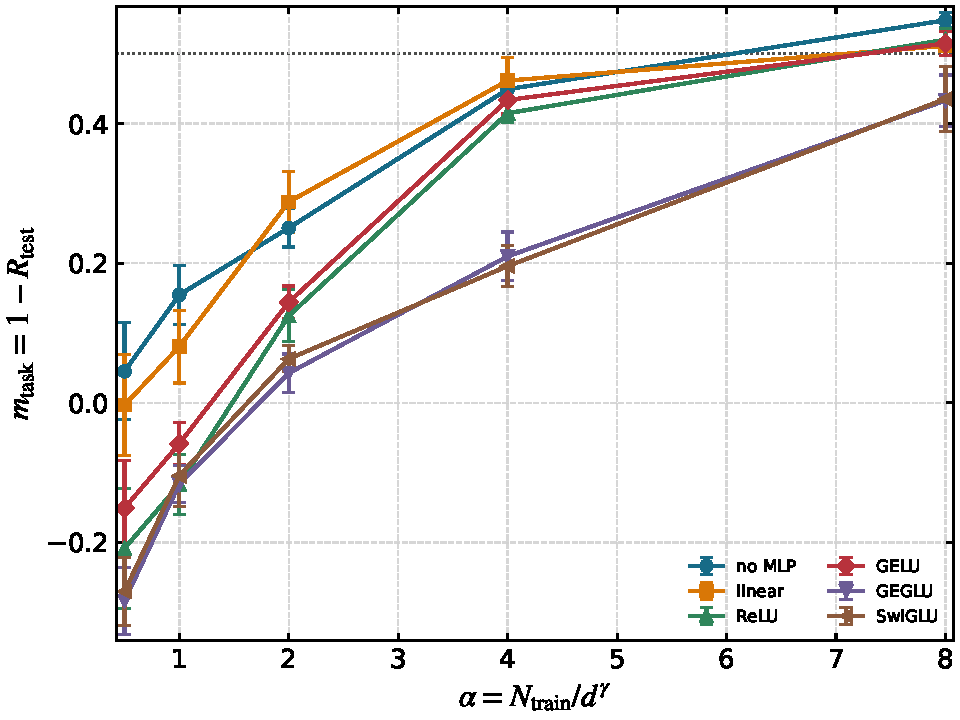
\includegraphics[width=0.94\linewidth]{figures/figure09_mlp_phase_splitting.pdf}
  \caption{MLP phase splitting at fixed attention, residual parameterization,
  and data source. Points are five-seed means and bars are 95\% Student-$t$
  intervals.}
  \label{fig:tensor-mlp-phase}
\end{figure}}{}

\IfFileExists{figures/figure10_mlp_causal_contribution.pdf}{
\begin{figure}[t]
  \centering
  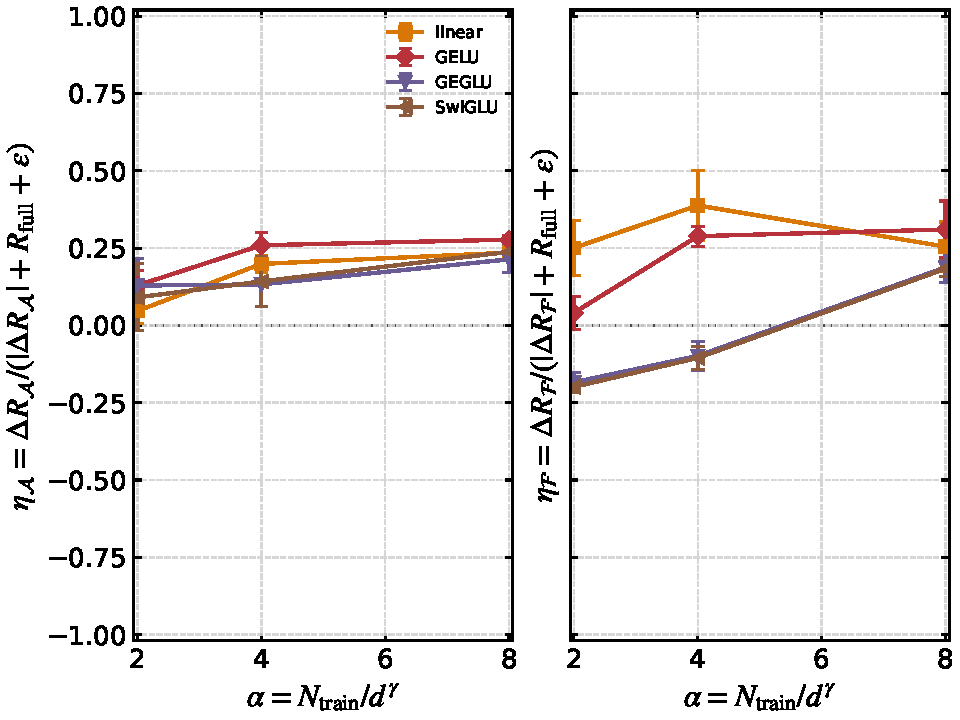
\includegraphics[width=0.94\linewidth]{figures/figure10_mlp_causal_contribution.pdf}
  \caption{Paired MLP ablation contribution across the sample continuation.}
  \label{fig:tensor-mlp-causal}
\end{figure}}{}

\IfFileExists{figures/figure11_optimizer_geometry.pdf}{
\begin{figure}[t]
  \centering
  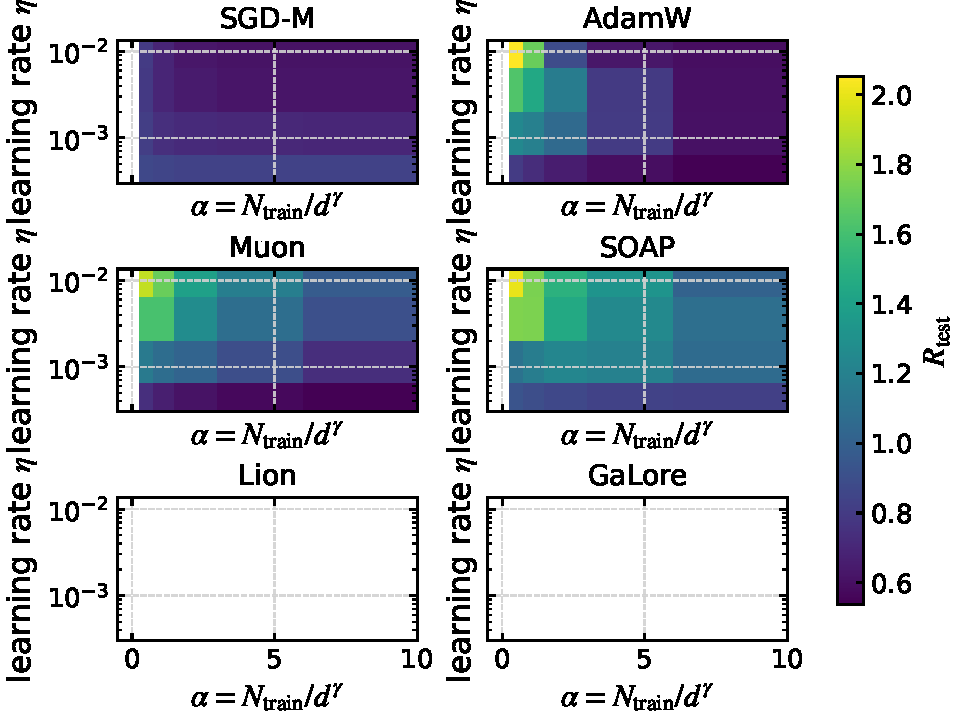
\includegraphics[width=0.94\linewidth]{figures/figure11_optimizer_geometry.pdf}
  \caption{Optimizer--normalization response surfaces for intensive held-out
  risk. Learning rate is treated as a swept coordinate.}
  \label{fig:tensor-optimizer}
\end{figure}}{}

\IfFileExists{figures/figure12_optimizer_gradient_heterogeneity.pdf}{
\begin{figure}[t]
  \centering
  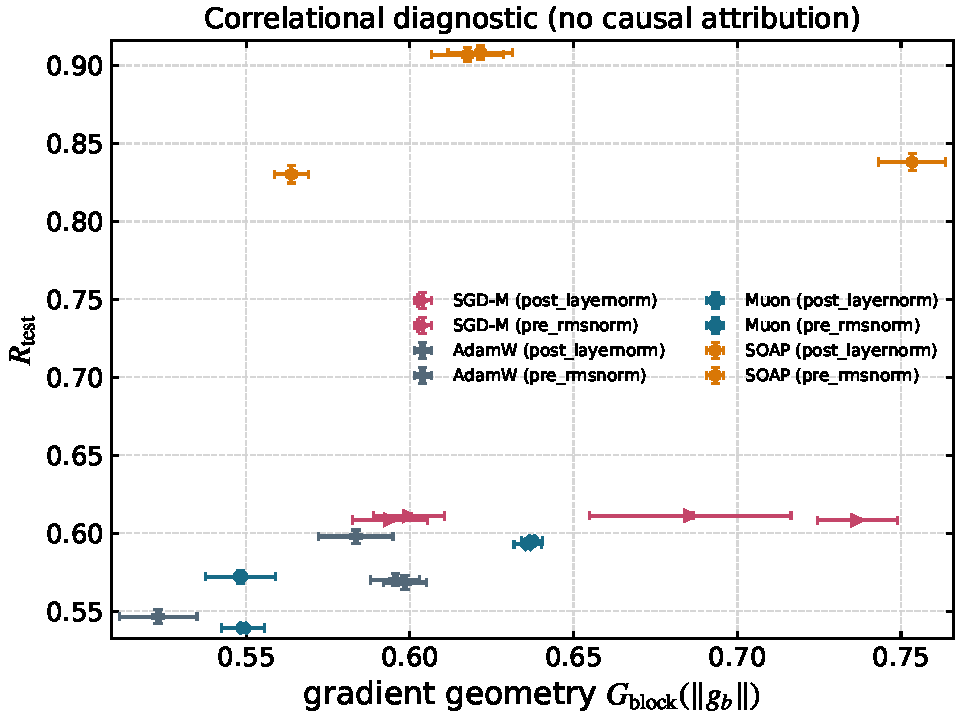
\includegraphics[width=0.94\linewidth]{figures/figure12_optimizer_gradient_heterogeneity.pdf}
  \caption{Gradient-block heterogeneity under optimizer and normalization
  continuation.}
  \label{fig:tensor-gradients}
\end{figure}}{}

\IfFileExists{figures/figure13_objective_homotopy.pdf}{
\begin{figure}[t]
  \centering
  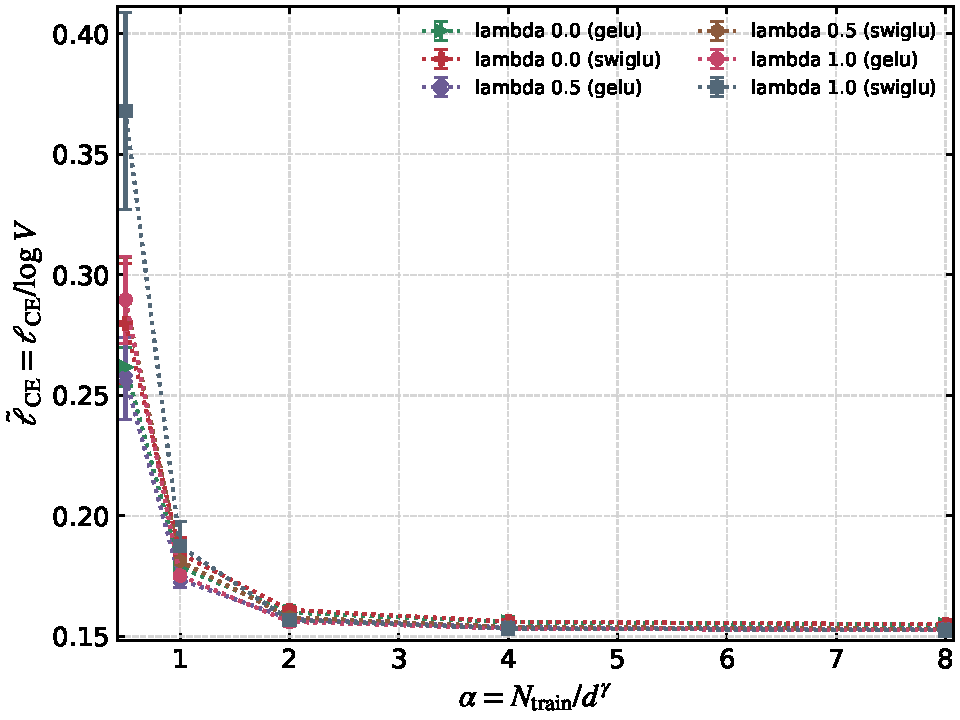
\includegraphics[width=0.94\linewidth]{figures/figure13_objective_homotopy.pdf}
  \caption{Objective homotopy crossed with MLP nonlinearity.}
  \label{fig:tensor-objective}
\end{figure}}{}

\IfFileExists{figures/figure14_scaling_paths.pdf}{
\begin{figure}[t]
  \centering
  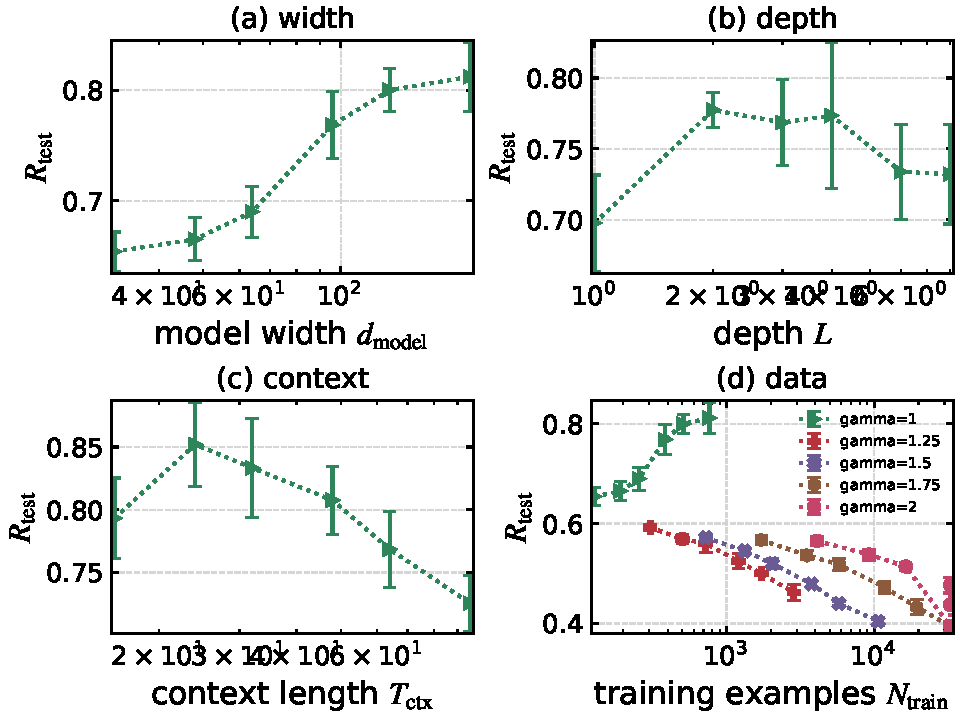
\includegraphics[width=0.94\linewidth]{figures/figure14_scaling_paths.pdf}
  \caption{Width, depth, context, and data are retained as distinct scaling
  paths rather than collapsed onto parameter count.}
  \label{fig:tensor-scaling}
\end{figure}}{}

\IfFileExists{figures/figure15_natural_data_bridge.pdf}{
\begin{figure}[t]
  \centering
  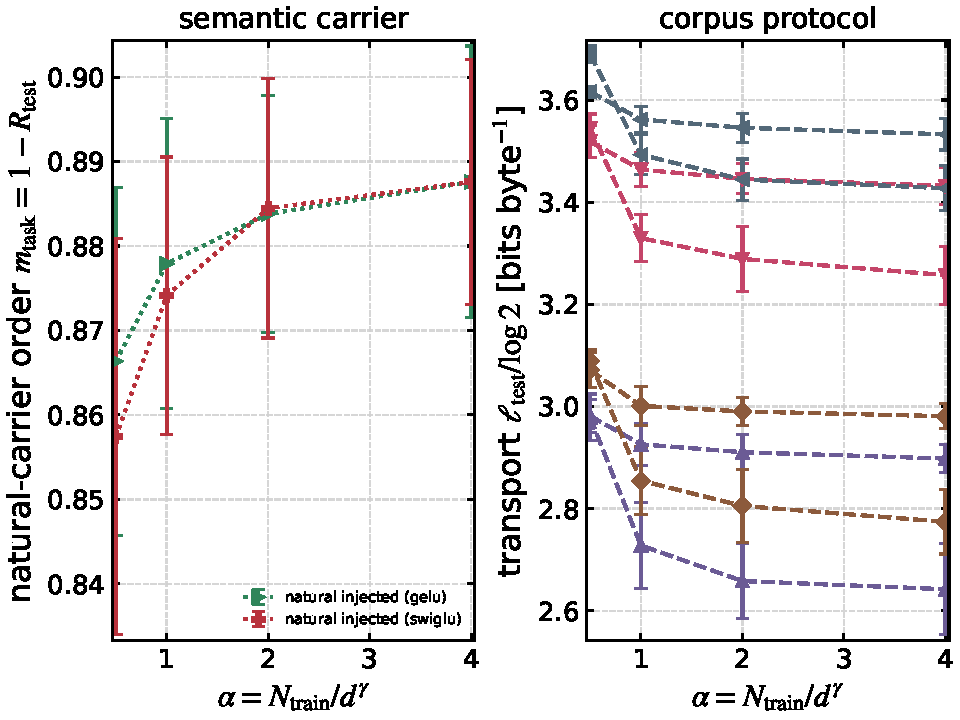
\includegraphics[width=0.94\linewidth]{figures/figure15_natural_data_bridge.pdf}
  \caption{Natural-data bridge in tokenizer-independent bits per byte.}
  \label{fig:tensor-natural-bpb}
\end{figure}}{}

\IfFileExists{figures/figure16_natural_data_generalization.pdf}{
\begin{figure}[t]
  \centering
  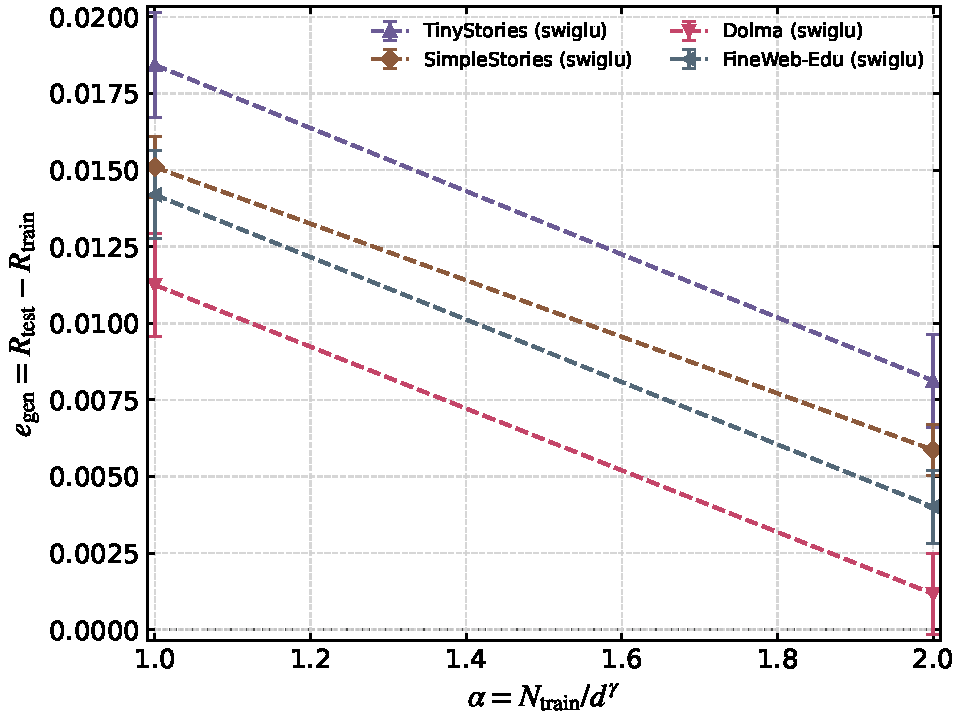
\includegraphics[width=0.94\linewidth]{figures/figure16_natural_data_generalization.pdf}
  \caption{Generalization gap $e_{\rm gen}=R_{\rm test}-R_{\rm train}$ across
  semi-natural and natural-data regimes.}
  \label{fig:tensor-natural-generalization}
\end{figure}}{}

\IfFileExists{figures/figure17_compute_error_landscape.pdf}{
\begin{figure}[t]
  \centering
  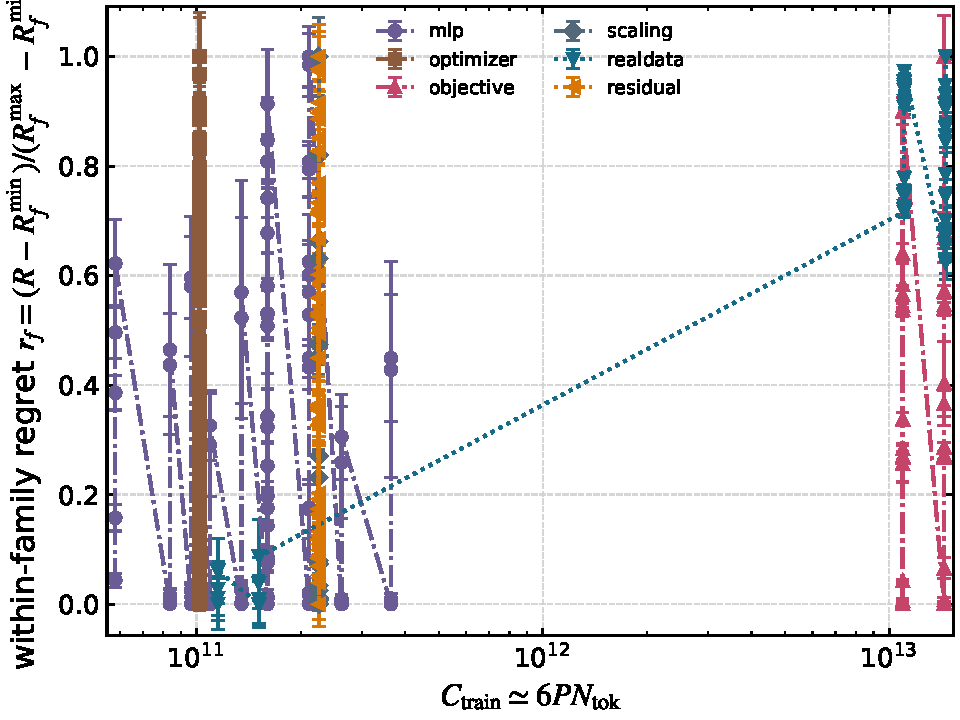
\includegraphics[width=0.94\linewidth]{figures/figure17_compute_error_landscape.pdf}
  \caption{Audited compute--error landscape. FLOPs remain an extensive resource
  coordinate; the vertical axis is an intensive risk.}
  \label{fig:tensor-compute}
\end{figure}}{}

\IfFileExists{figures/figure18_theory_experiment_coverage.pdf}{
\begin{figure}[t]
  \centering
  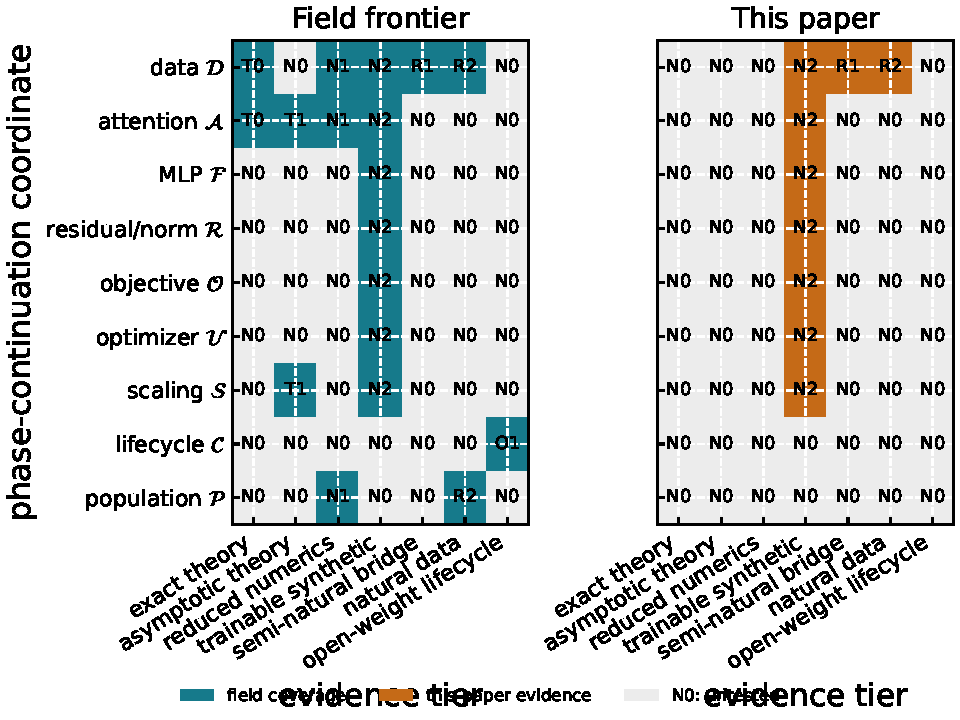
\includegraphics[width=0.94\linewidth]{figures/figure18_theory_experiment_coverage.pdf}
  \caption{Theory--experiment coverage of the nine-axis tensor. Grey N0 cells
  are declared untested rather than omitted.}
  \label{fig:tensor-coverage}
\end{figure}}{}

\IfFileExists{figures/figure19_training_generalization_dynamics.pdf}{
\begin{figure}[t]
  \centering
  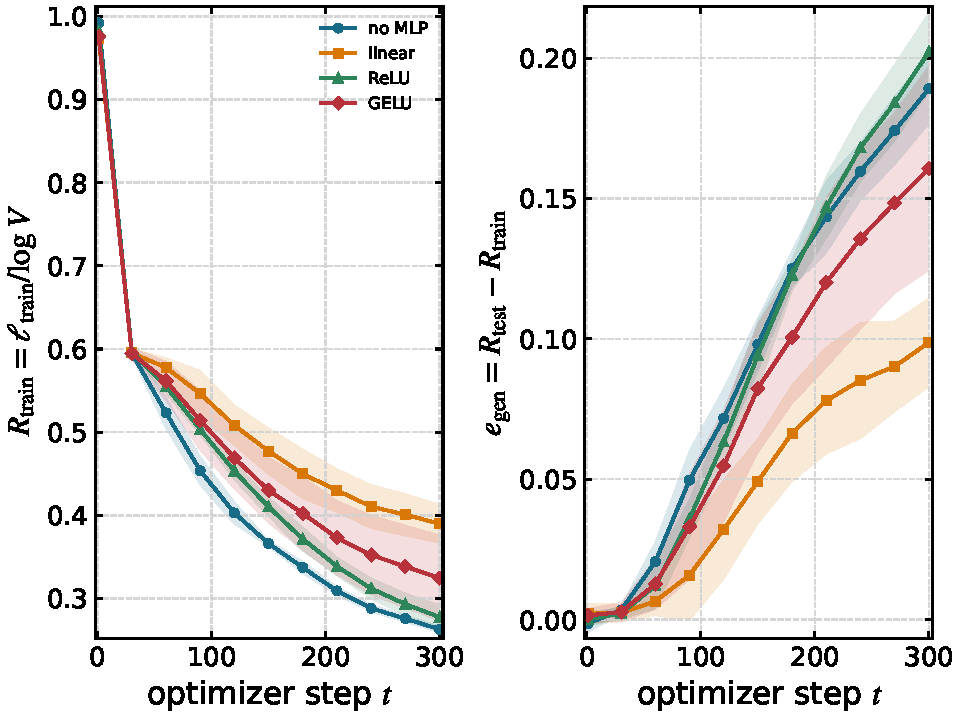
\includegraphics[width=0.94\linewidth]{figures/figure19_training_generalization_dynamics.pdf}
  \caption{Five-seed training dynamics. Training risk and the generalization gap
  are separate $O(1)$ observables; shaded bands are 95\% Student-$t$ intervals.}
  \label{fig:tensor-dynamics}
\end{figure}}{}

\IfFileExists{figures/figure20_mlp_mechanism_atlas.pdf}{
\begin{figure}[t]
  \centering
  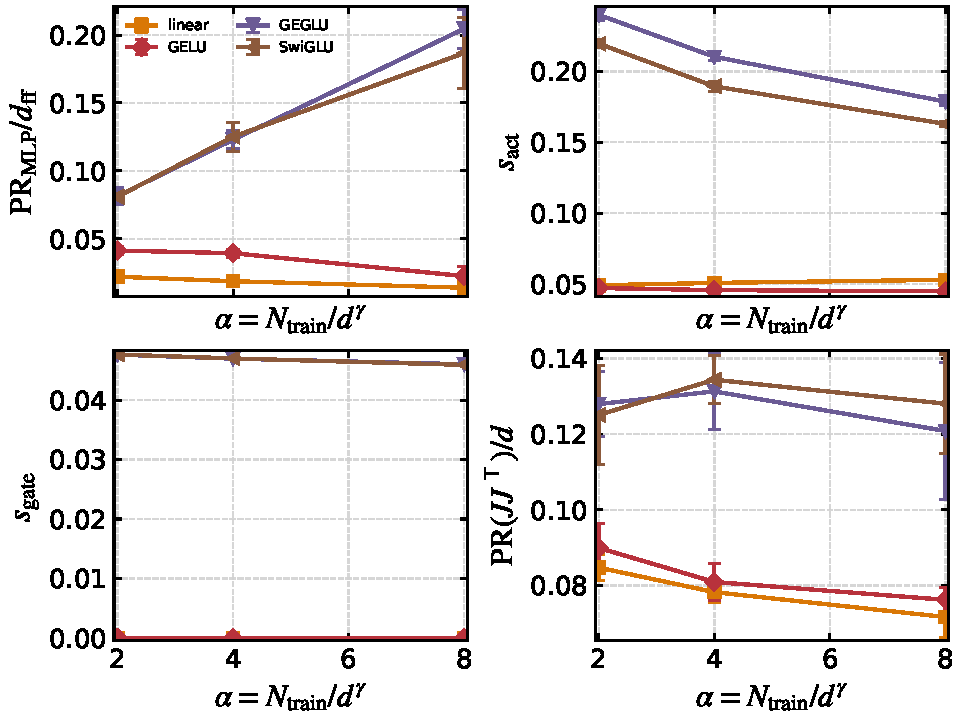
\includegraphics[width=0.94\linewidth]{figures/figure20_mlp_mechanism_atlas.pdf}
  \caption{MLP mechanism atlas. Effective rank, occupancy, and gate statistics
  are reported separately from task performance and causal contribution.}
  \label{fig:tensor-mlp-mechanism}
\end{figure}}{}

\clearpage
